\documentclass[8pt]{article}
\usepackage{amsmath}
\usepackage{amssymb}
\usepackage{amsthm}
% \usepackage{amsfonts}
% \usepackage{amscd}
\usepackage{graphicx}
\usepackage{color}
\usepackage{hyperref}
\usepackage{enumerate}
% \usepackage{mathrsfs}
% \usepackage{tikz}
% \usepackage{tikz-cd}
\usepackage{listings}
\usepackage{xcolor}
\usepackage{textcomp}
\usepackage{xcolor}
\usepackage{verbatim}
\usepackage{subfig}

% To define colors
\definecolor{commentgreen}{RGB}{40, 180, 20}
% \definecolor{commentgreen}{RGB}{2,112,10}
\definecolor{eminence}{RGB}{108,48,130}
\definecolor{weborange}{RGB}{255,160,180}
\definecolor{frenchplum}{RGB}{180,30,10}

% To EXTREMELY customiza the style of the listings package
\lstset{
    basicstyle=\ttfamily,
    columns=fullflexible,
    breaklines=true,
    breakatwhitespace=true,
    frame=single,
    framerule=0.1pt,
    framesep=5mm,
    showstringspaces=false,
    showspaces=false,
    showtabs=false,
    tabsize=4,
    % numbers=left,
    numberstyle=\tiny,
    numbersep=5pt,
    stepnumber=1,
    numberblanklines=true,
    captionpos=b,
    backgroundcolor=\color{gray!10},
    keywordstyle=\color{weborange}, %\bfseries\underbar
    commentstyle=\color{commentgreen},
    stringstyle=\color{red},
    % identifierstyle=\color{pink},
    emph={as, from}, emphstyle=\color{weborange},
    % emph={[2]import}, emphstyle={[2]\color{blue}},
    breakautoindent=true,
    breakindent=2em,
    keepspaces=true,
    morekeywords={for, while, if, else, elif, def, return, print, in, range, len, enumerate, zip, list, tuple, set, dict, True, False, None, and, or, not, is, in, not in, from, import, as, try, except, finally, raise, assert, pass, del, global, nonlocal, lambda, with, yield, class, break, continue, async, await},
    xleftmargin=1.5cm,
    xrightmargin=1.5cm,
    frameround=tttt,
    rulecolor=\color{gray!40},
    % To make bigger the radius of the frame:
    frameround=2mm,
}

% To EXTREMELY customiza the style of the verbatim inline
\newcommand{\code}[1]{\texttt{\color{frenchplum}{#1}}}

% Margins = 2cm and 4cm
\usepackage[margin=2cm, left=4cm, right=4cm]{geometry}

% Fonts and language in Spanish
\usepackage[spanish]{babel}
\usepackage[utf8]{inputenc}

% Rename things
\renewcommand{\contentsname}{Contenido}
\renewcommand{\sectionautorefname}{Sección}
\renewcommand{\subsectionautorefname}{Subsección}
\renewcommand{\subsubsectionautorefname}{Subsubsección}
\renewcommand{\figureautorefname}{Figura}
\renewcommand{\tableautorefname}{Tabla}
\renewcommand{\equationautorefname}{Ecuación}
\renewcommand{\appendixautorefname}{Apéndice}
\renewcommand{\appendixname}{Apéndices}

\title{Teoremas del límite: ley de los grandes números y teorema límite central}
\author{Jorge Antonio Gómez García \\ Saud Antonio Morales González}
\date{\today}


% ##################################################################


\begin{document}
\maketitle
\tableofcontents
\pagebreak


% ##################################################################


\section{Introducción}
TEXT ...............................................................


% ##################################################################

\section{Ley de los grandes números}

% ##################################################################

\subsection{Ley débil de los grandes números}

Sea $X_i$ una secuencia de variables aleatorias independientes tales que $\text{E}[X_i] = \mu$ y $\text{var}(X_n) \leq M$ para todo $n \geq 1$. Entonces, la siguiente secuencia de variables aleatorias converge a $\mu$ en probabilidad:

\begin{align*}
    \overline{X}_n &:= \frac{1}{n}(X_1 + \cdots + X_n) = \frac{1}{n}\sum_{i=1}^n X_i \longrightarrow \mu \quad \text{en probabilidad}.
\end{align*}

De esta ecuación tenemos que:

\begin{align*}
    \text{E}[\overline{X}^2_n] &\rightarrow \mu^2 \\
\end{align*}

\subsubsection{Ejemplo en Python}

Considere el siguiente ejemplo: Sean $X_1, X_2, \ldots$ variables aleatorias independientes con distribución exponencial, tal que $X_i \sim \text{Exp}(\lambda)$. El segundo momento $\text{E}[\overline{X}^2_i]$ de $X_i$, con $m$ diferentes valores de $\omega$, puede ser simulado en Python de la siguiente manera:

\vspace*{0.3cm}

Importamos las librerías necesarias y definimos los parámetros:

\begin{lstlisting}[language=Python]
# Librerias
import numpy as np
import matplotlib.pyplot as plt

# Parametros
media_exp = 2   # beta = 0.5
n = 10000       # Numero de variables aleatorias
m = 50          # Numero de w's
\end{lstlisting}

Generamos $m$ muestras de $n$ variables aleatorias con distribucion exponencial:

\begin{lstlisting}[language=Python]
x = np.random.exponential(media_exp, (m,n))
    # (m,n) es una matriz (filas, columnas)
\end{lstlisting}

Obtenemos la media de cada una de las muestras:

\begin{lstlisting}[language=Python]
x_barra = np.mean(x, axis=1)
    # axis=1: calcula la media de cada fila
    # (m, 1) es un vector columna
\end{lstlisting}

Obtenemos el segundo momento de cada una de las muestras:

\begin{lstlisting}[language=Python]
x_barra_cuadrado = np.mean(x_barra**2)

print(x_barra_cuadrado)
    # 4.0000000000000004
\end{lstlisting}

\vspace*{0.3cm}

¿Qué describe el código anterior? Primero, determinamos los parámetros de la distribución exponencial. En este caso la media está definida como \code{media\_exp = 2}. Luego, generamos \code{m} muestras de \code{n} variables aleatorias con distribución exponencial. Finalmente, calculamos el segundo momento de cada una de las muestras. En este caso, el segundo momento es \code{4.0000000000000004}.




% ##################################################################

\subsection{Ley fuerte de los grandes números}



% ##################################################################

\section{Teorema límite central}

Sean $X_1, X_2, ..., X_n$ n variables aleatorias IID con una distribucion de probabilidad no específicada y que tienen una media $\mu$ y una varianza $\sigma^2$ finita. El promedio muestral $\overline{X} = (X_1, X_2, ..., X_n)/n$ tiene una distribución con media $\mu$ y varianza $\sigma^2/n$ que tiende hacia una distribución normal conforme $n$ tiende a $\infty$. En otras palabras, la variable aleatoria $(\overline{X}-\mu)/(\sigma/\sqrt{n})$ tiene como limite una distribución normal estándar.\footnote{George C. Canavos, \textit{Probabilidad y estadística: aplicaciones y métodos}, trad. Edmundo Urbina (Ciudad de México: McGraw Hill, 1988), 230.} 

La demostración de este teorema puede ser consultada en las páginas 247-249 del libro de \textit{Probabilidad y estadística: aplicaciones y métodos} de George Canavos.

\subsection{Teorema de Moivre-Laplace}

Sea $X$ una variable aleatoria binomial con media $np$ y desviación estandar $\sqrt{np(1-p)}$. La distribución de la variable aleatoria tiende a la normal estandar conforme el número de ensayos independientes $n \rightarrow \infty$. \footnote{Canavos, \textit{Probabilidad y estadística: aplicaciones y métodos}, 141-142.} En otras palabras, una distribución binomial tenderá a la normal estándar conforme el número de ensayos vaya aumentando.

\
Para ilustrarlo se graficaran las funciones de masa de probabilidad de que una moneda caiga cara en $n$ experimentos. Donde $n$ tomará valores cada vez más grandes.\

\begin{figure}
        \subfloat[n=5]{
            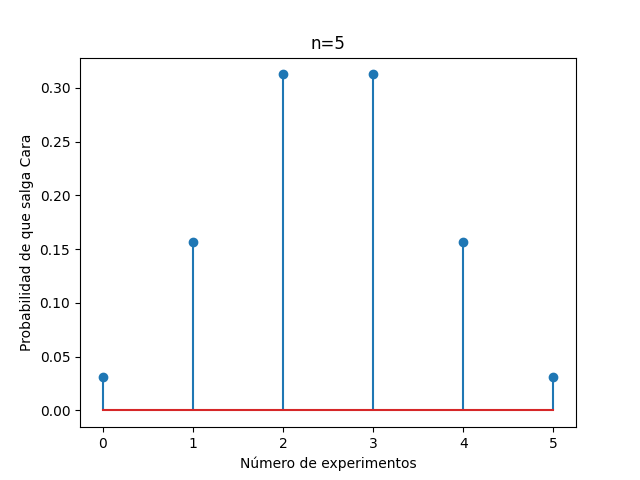
\includegraphics[scale=.4]{n=5.png}}
        \subfloat[n=10]{
            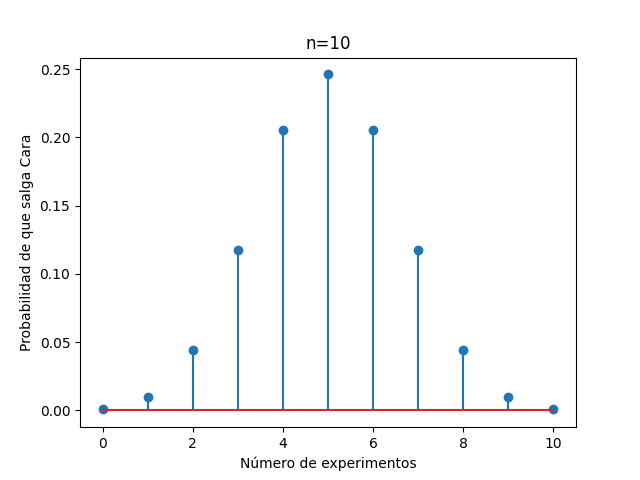
\includegraphics[scale=.4]{n=10.png}}\\
        \subfloat[n=30]{
            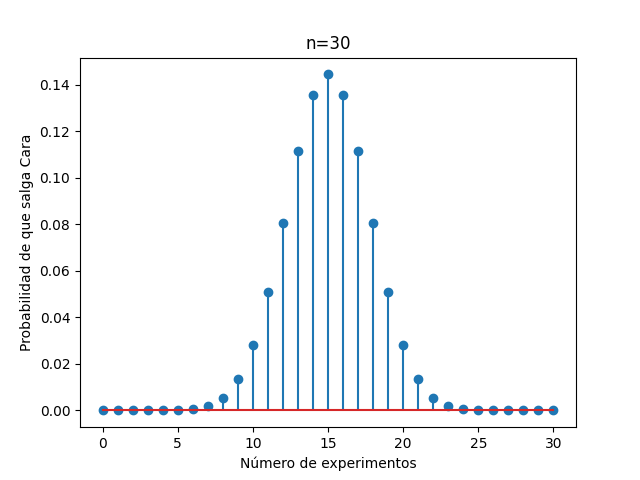
\includegraphics[scale=.4]{n=30.png}}
        \subfloat[n=50]{
            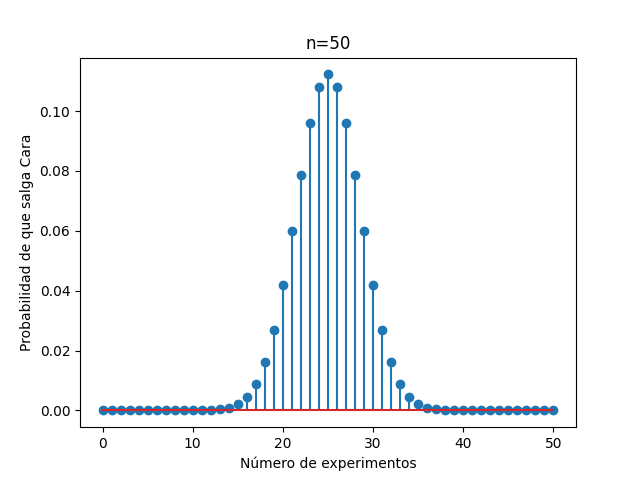
\includegraphics[scale=.4]{n=50.png}}\\
        \subfloat[n=100]{
            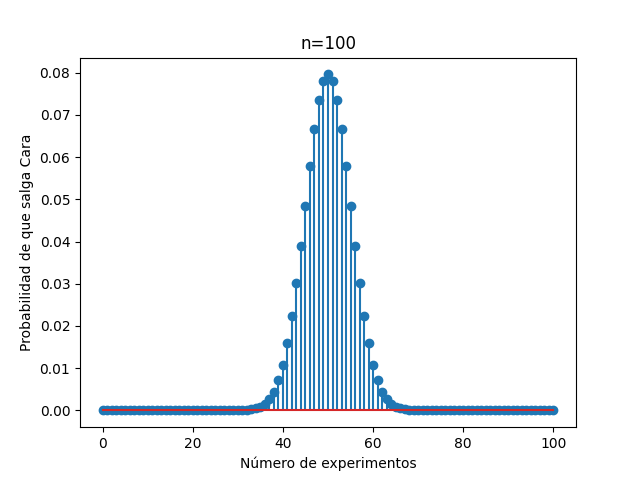
\includegraphics[scale=.4]{n=100.png}}
        \subfloat[n=500]{
            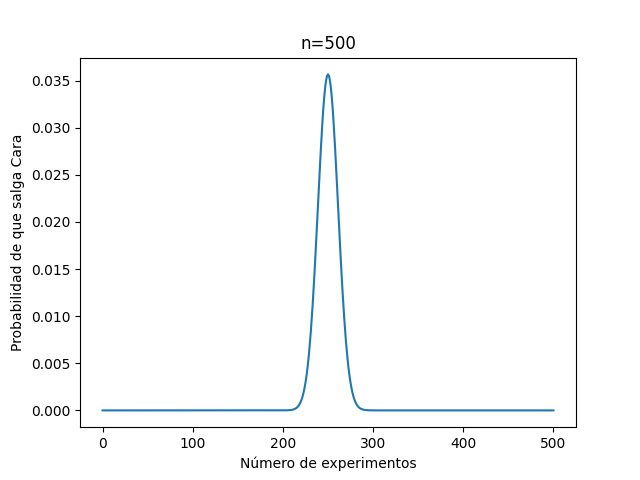
\includegraphics[scale=.4]{n=500.png}}
        \caption{Teorema de Moivre-Laplace}
        \label{f:animales}

\end{figure}

\
Como es observado, mientras más aumenta la cantidad de experimentos realizados, más se asemeja la función de masa de probabilidad de la distribución binomial a la función de densidad de probabilidad de la distribución normal.


\end{document}